\chapter{Conclusion}\label{chapter:conclusion}
We have successfully formalized the \textbf{NP-Hardness} of 
a few selected classical decision problem.  
The whole work consists of 3834 lines of codes, with which we add 
six new problems into the Karp21 project. A general overview of the 
progress of the list is given in the following graph.\\\\
The new reductions from this work are given as red arrows. 
It is also noticed that a reduction from \SAT\ to \textbf{3CNF-Satisfiability} is not 
formalized yet, and is an interesting work in the future. With this work,
we manage to show the possibility of formalising and verifying the polynomial 
reductions and to provide a theorectical basis for other works related 
to the complexity theory, especially the NP-Hardness. 
\begin{figure}[h!]
\centering 
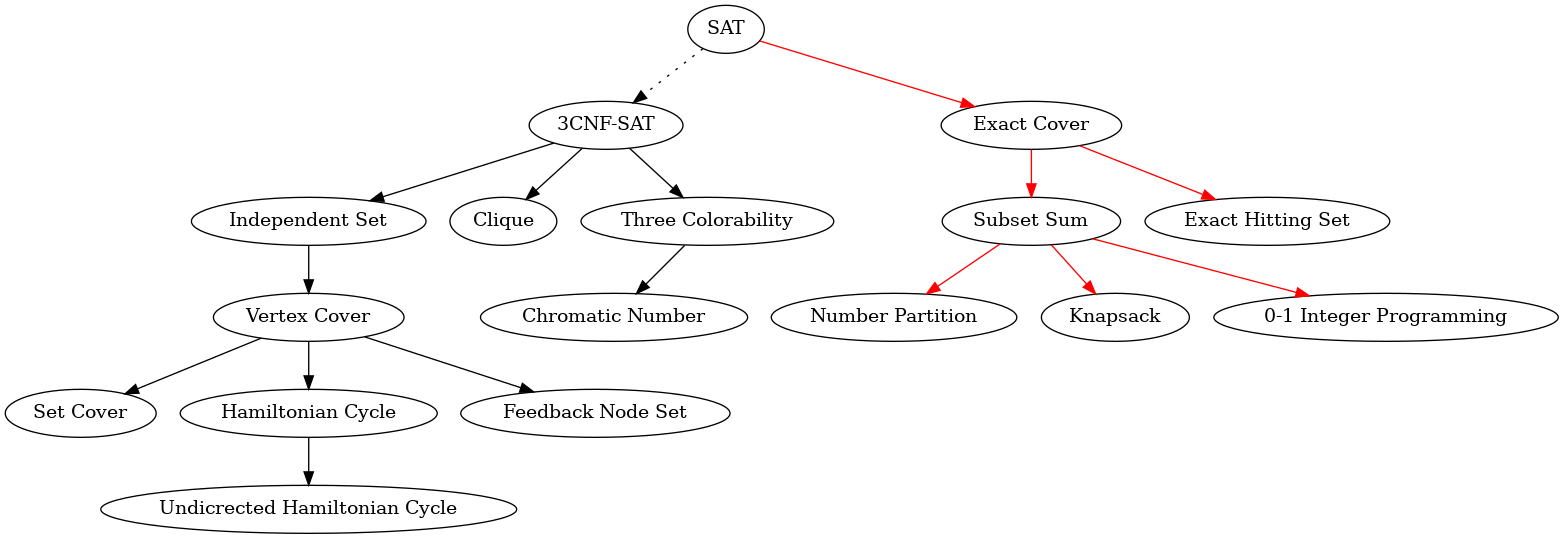
\includegraphics[angle = 90, scale=0.39]{figures/reductions_new.png}
\caption{The updated reduction graph of the Karp21 project.}
\end{figure}

\section*{Future Work}
As a future work, it is necessary to add a few new reductions and complete Karp's 
list of twenty-one NP-hard problems. We summarize the remaing problems as follows,
\begin{enumerate}
    \item 3cnf-satisfiability, feedback arc set, clique cover. Reductions to these problems 
    are not related to this work. Reductions are strongly dependent on the previous works.
    \item 3-dimensional match, steiner tree, job sequencing, max cut. The reductions 
    presented by Karp are dependent on this work. Unfortunately, the definition of these problems 
    are significantly different from the existing problems. Thus, the reductions
    from the existing problems may not be straightforward and can be replaced by 
    a better one.
\end{enumerate}
Furthermore, a few other classical NP-Hard problems that are not in Karp's list 
can also be added to Karp21 project. Traveling salesman problem, for example, 
can be reduced from Hamilton's circuit, while the bin packing problem is also 
reducible from the partition. 
